\chapter{FtsZ: function and structure}\label{ftsz}

To better understand the role of FtsZ in the septation of \textit{D. radiodurans}, we investigated its structure and superstructure using both single particle cryo-EM and \textit{in situ} cryo-ET.
This work is ongoing and not yet consolidated into a manuscript for publication.

\localtableofcontents

\section{Introduction}

As mentioned in \fullref{drad_ftsz}, FtsZ is an extremely well conserved prokaryotic tubulin homologue, known to form ring-like structures (the Z-ring) at the septation site in most bacteria.
It polymerizes in a GTP-dependent fashion to form filaments and bundles, anchoring to the membrane via its partner FtsA, and interacting with several other partners in the cytokinesis and peptidoglycan (PG) synthesis machinery~\cite{barrowsFtsZDynamicsBacterial2021,mcquillenInsightsStructureFunction2020}.

Based on crystal structures, filaments have been shown to form through head-to-tail stacking of monomers CITE.
However, there is no structural information regarding the flexible C-terminal region, which is responsible for regulating its activity and interaction with its cellular partners, including FtsA.
It's also unclear how multiple filaments may assemble to form bundles at the structural level and even less so in vivo.
Thus --- while its key role in cell division is undisputed --- the exact mechanism and function of FtsZ are still unclear.
There is no consensus model, as the current evidence is inconclusive, sometimes presenting significant variations between species --- likely ascribable to different shapes or membrane compositions between bacteria~\cite{barrowsFtsZDynamicsBacterial2021,mcquillenInsightsStructureFunction2020}.

\begin{figure}[ht]
    \centering
    \includegraphics[width=.5\textwidth]{example-image.png}
    \titledcaption{TODO: ftsz ring and cystal structure?}
    \label{fig:ftsz_ring}
\end{figure}

Some studies have shown that FtsZ presents mechanical functions that may drive the septation process.
\textit{T. maritima} FtsZ+FtsA expressed in liposomes was shown to form coil-like structures, which can constrict the membrane via a "filament sliding" mechanism, creating a partial septum~\cite{szwedziakArchitectureRingFormed2014}.
In \textit{C. crescentus}, FtsZ may form short, loosely bundled filaments, which may drive constriction via an "iterative pinching" mechanism where repeated rounds of phosphorylation lightly bend the filament, thus slowly pinching the membrane~\cite{liStructureFtsZFilaments2007}.

Other publications investigated the recruitment and signalling role of FtsZ for downstream machinery such as PG synthesis.
FtsZ was shown to undergo plus-end polymerization and minus-end depolymerization, in a GTP-regulated process typical of cytoskeletal proteins called treadmilling~\cite{looseBacterialCellDivision2014}.
In \textit{B. subtilis}, this treadmilling is required to drive the movement along the septum of the PG synthesis centers~\cite{bisson-filhoTreadmillingFtsZFilaments2017}.
A "diffusion-and-capture" model was proposed, where the FtsZ ring performs a recruitment role by engaging in weak transient interactions with downstream machinery for PG synthesis~\cite{baranovaDiffusionCapturePermits2020}.
However, in \textit{S. aureus}, cytokinesis may actually occur in two separate steps: a slow, FtsZ-driven, treadmilling-dependent step which causes initial invagination, followed by a faster step where PG synthesis is the driving force for septation~\cite{monteiroPeptidoglycanSynthesisDrives2018}.

While FtsZ ring formation and PG synthesis are clearly linked, their precise interaction may differ between bacteria.
In \textit{E. coli}, GTP regulates FtsZ treadmilling, which in turn controls the movement of the synthesis machinery~\cite{yangGTPaseActivityCoupled2017}.
However, it does not appear to affect the rate of PG synthesis, as opposed to what happens in \textit{B. subtilis}, which suggest that the presence or absence of an outer membrane may change PG synthesis machinery regulation~\cite{yangGTPaseActivityCoupled2017}.
Indeed, in \textit{E. coli}, some additional proteins may help with a timely invagination of the outer membrane, although they are not needed for septation to occur~\cite{gerdingTransenvelopeTolPal2007}.
This is intriguing for \textit{D. radiodurans} which, despite staining gram-positive, presents an outer membrane.

The disordered C-terminal domain of FtsZ was found the be necessary both for the anchorage to the membrane via FtsA, and to regulate oligomerization as well as bundling with neighboring filaments~\cite{barrowsFtsZDynamicsBacterial2021}.

Collectively, the literature hints that FtsZ treadmilling is likely not the only factor that controls the dynamics of FtsZ and the Z-ring, and that variations across species may be explained by different divergent mechanisms, or some other underlying behavior not yet discovered~\cite{barrowsFtsZDynamicsBacterial2021}.

\section{Results}

\subsection{Structural study by SPA}

To begin our investigation of the structure of DrFtsZ, prepared a sample for SPA from \textit{in vitro} purified FtsZ.
The preparation we selected (\fullref{ftsz_methods}) resulted in FtsZ filaments long enough to allow filament picking and helical reconstruction, while avoiding an excess of filament bundles which make picking and refinement more difficult (\autoref{fig:ftsz_micrographs}).
It was tricky to strike the balance between 

.. TODO: how was it prepared exactly? concentrations, wait time for polymerization, ...


\begin{figure}[ht]
    \centering
    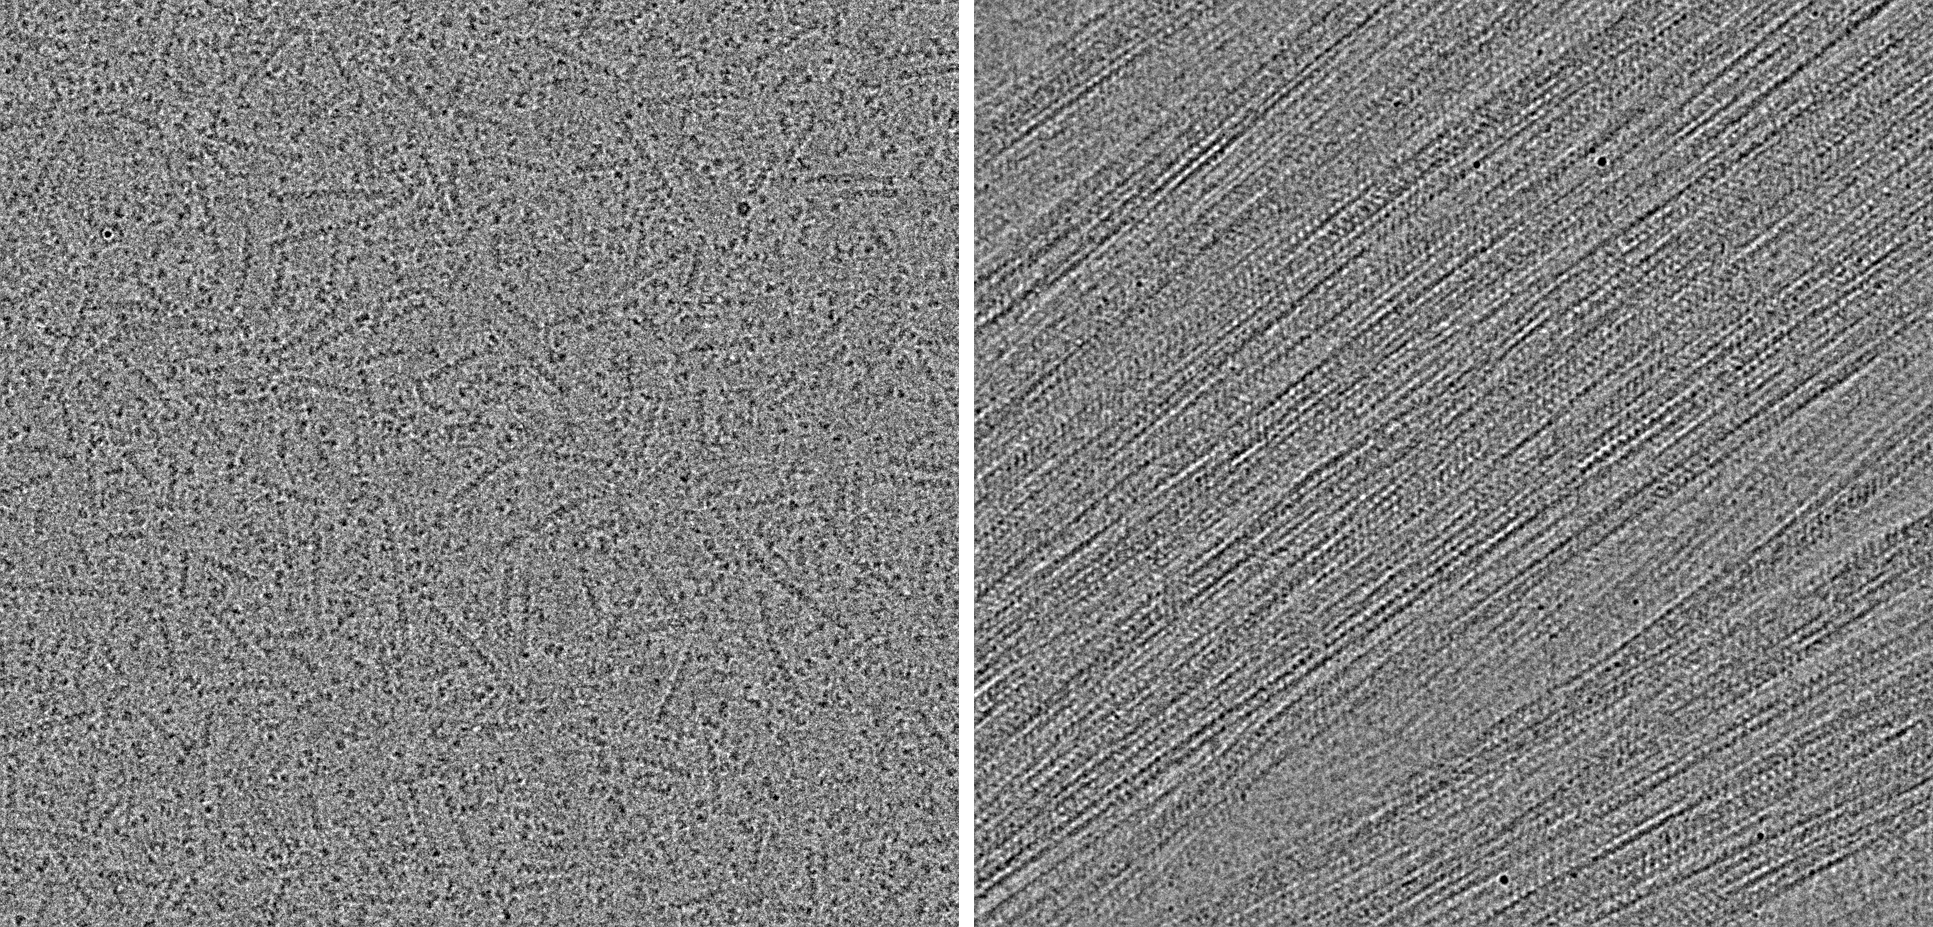
\includegraphics[width=\textwidth]{other/ftsz_mics.png}
    \titledcaption[Micrographs of FtsZ filaments]{Micrographs containing FtsZ filaments. When filaments are well separated (left) they are ideal for picking and refinement. In some cases, FtsZ filaments form bundles (right) which are harder to pick, refine and classify due to the overlapping particles.}
    \label{fig:ftsz_micrographs}
\end{figure}

We used CryoSPARC~\cite{punjaniCryoSPARCAlgorithmsRapid2017} for filament picking, which gave us a large amount of particles (>4M) to classify and clean up from spurious picks.
After cleaning, we ended up with about 2M particles, and very uniform classes with little variation (\autoref{fig:ftsz_classes}).
This is a typical symptom of strong preferential orientation due to the air-water interface (\fullref{em_pref_ori}), leading to a very limited range of views in the particle projections.
Though we saw hints of different views in the bundled filaments, they proved impossible to disentangle enough to obtain well-resolved classes.

\begin{figure}[ht]
    \centering
    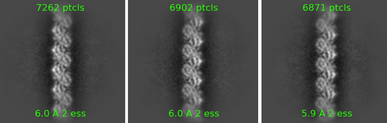
\includegraphics[width=\textwidth]{other/ftsz_classes_untilted.png}
    \titledcaption[FtsZ filament: 2D classes]{Classification results from particles with strong preferential orientation. All classes show very similar views of the FtsZ filaments, with minor variation in the out-of-plane angle.}
    \label{fig:ftsz_classes}
\end{figure}

Given the strong preferential orientation, it's unsurprising that 3D reconstructions from these particles showed very strong resolution anisotropicity (while reporting \sim4 Å global resolution), so much so that we couldn't convincingly fit the monomeric model in the map (\autoref{fig:ftsz_map_bad}).

\begin{figure}[ht]
    \centering
    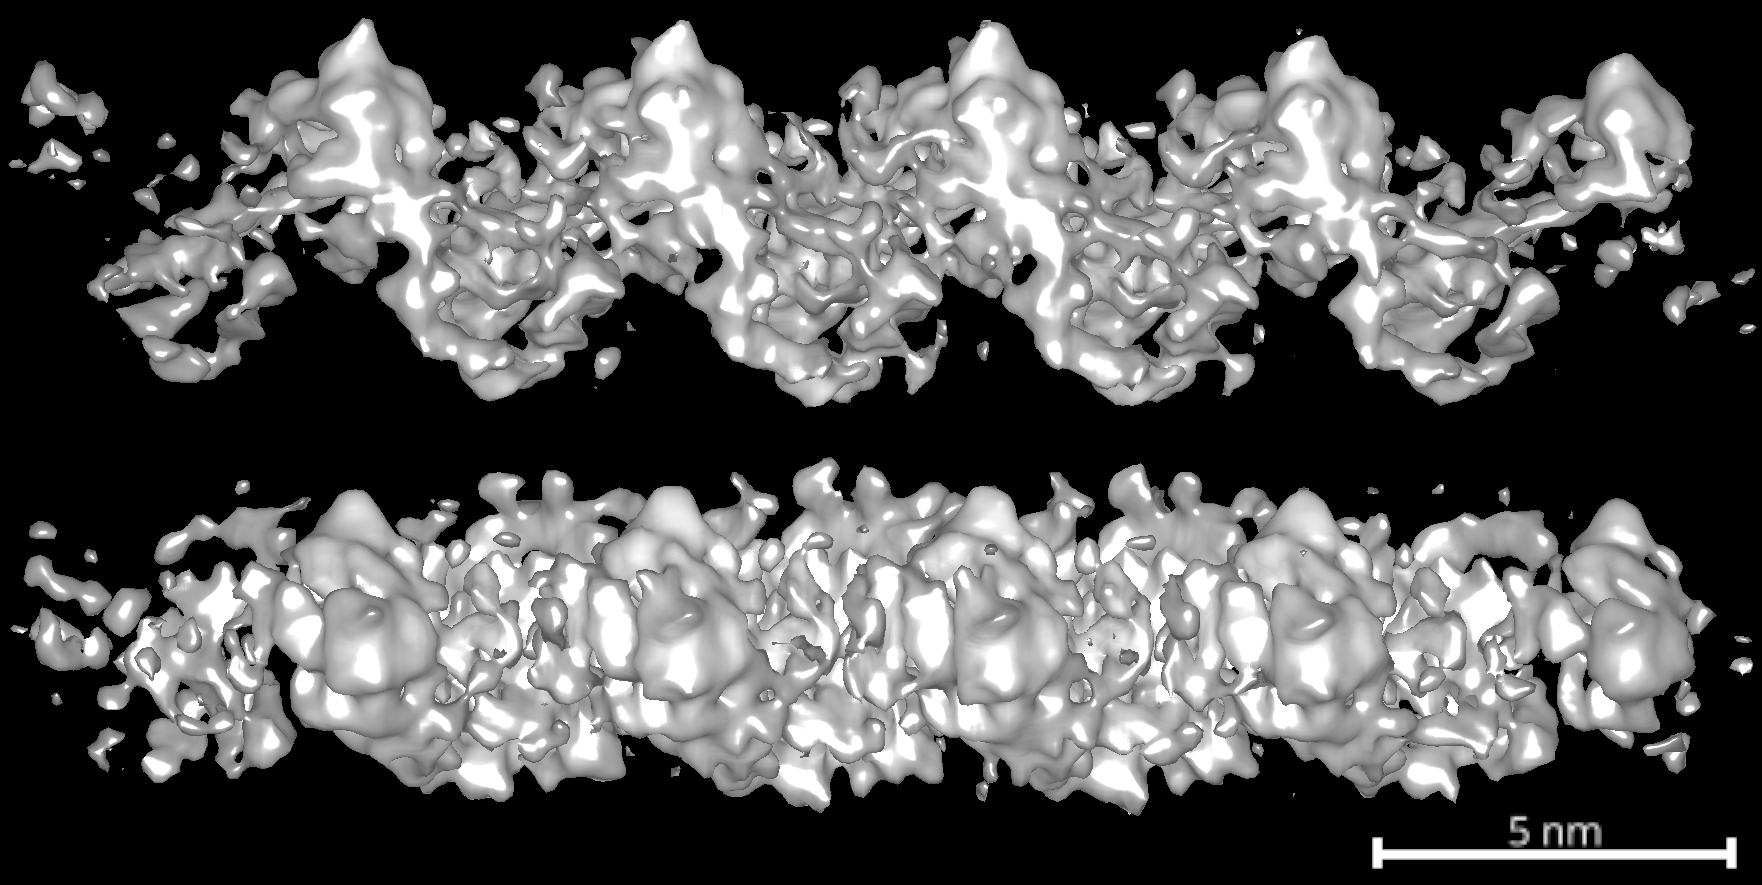
\includegraphics[width=\textwidth]{other/ftsz_map_bad.png}
    \titledcaption[FtsZ filament: anisotropic map]{FtsZ filament map affected by preferential orientation, viewed from the same direction as most 2D classes (top) and rotated by 90° (bottom) to highlight the streaking artifacts due to anisotropic orientation sampling.}
    \label{fig:ftsz_map_bad}
    % TODO: add pref orientation proof (orientation map or so)
\end{figure}

The best map available of FtsZ filaments (from \textit{Klebsiella pneumoniae}) also suffered from similar issues, despite high reported resolution (\sim3 Å)~\cite{fujitaStructuresFtsZSingle2023}.

We attempted to address the issue of preferential orientation in two different ways: collecting a tilted dataset of the same samples, and preparing a new sample with methods that combat air-water interface effects.

\subsubsection{Tilted dataset}\label{ftsz_tilted}

We prepared the sample in the same way, but this time the data collection was done with a 35° tilt.
Following the same workflow as with the untilted dataset, we then picked, classified and selected particles, obtaining a more promising selection of class averages (\autoref{fig:ftsz_classes_tilted}).

\begin{figure}[ht]
    \centering
    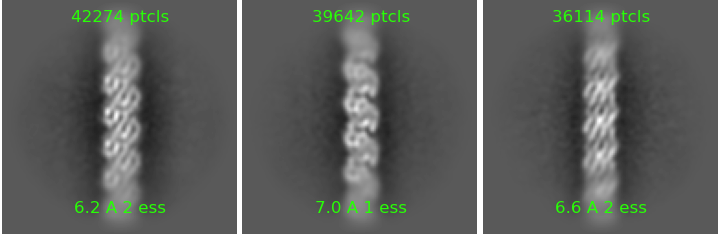
\includegraphics[width=\textwidth]{other/ftsz_classes_tilted.png}
    \titledcaption[FtsZ tilted dataset: 2D classes]{Classification results from the tilted dataset. Differently from the untilted classes, particles successfully classified into distinct views of the filament.}
    \label{fig:ftsz_classes_tilted}
\end{figure}

Despite the better view distribution of 2D classes, our 3D reconstructions had the same anisotropicity issues as the untilted data.
Assuming a unform distribution of in-plane angles of the filaments (which we observed in the original dataset), a single, relatively high-tilt dataset should cover a higher portion of 3D fourier space during backprojection and thus significantly improve map isotropicity~\cite{tanAddressingPreferredSpecimen2017}.

With preferentially oriented filament collected at a fixed tilt angle, there should be a strong correlation between in-plane angle (easily identifiable from the micrograph) and the projection view (which is identified by classification). % TODO: show with synthetic dataset? Also, could it be that multiple euler combinations are redundant and correlation was just bad? How did I do this thing again?
Upon closer inspection of the picking data, however, we observed that the out-of-plane angles assigned to each particle showed no correlation with the assigned 2D class (\autoref{fig:ftsz_angle_dist}).

\begin{figure}[ht]
    \centering
    \includegraphics[width=.5\textwidth]{example-image.png}
    \titledcaption{Out-of-plane angle plotted against the assigned 2D class. TODO}
    \label{fig:ftsz_angle_dist}
\end{figure}

We soon realized that the 3D reconstruction routines of both Relion and CryoSPARC were struggling with assigning orientations, resulting in practically random orientations.
To impose more constraints on the refinement based on this prior knowledge on the geometry of the system, we calculated the theoretical orientation of each particle based on the in-plane angle (and assuming perfect preferential orientation), which we then used to initialize the particle poses (\fullref{stemia_angles}).



---

%However, it was recently shown that the effect of these issues on the final resolution can be rendered negligible with careful preprocessing~\cite{aiyerOvercomingResolutionAttenuation2024}.

\subsubsection{Detergent and other methods}

% Other methods are a bit more involved, such as the use of functionalized graphene grids~\cite{luFunctionalizedGrapheneGrids2022}, streptavidin-coated affinity support grids~\cite{crucifixImmobilizationBiotinylatedDNA2004,hanLongShelflifeStreptavidin2016}, but can offer more control over the orientation of the particles in the sample.

Strong pref. orientation, map doesn't look better/worse than ~\cite{fujitaStructuresFtsZSingle2023}.

work so far, classes

detergent + other tricks = now better angular distribution

width

filament picking...

\section{Tomography and STA}

(TODO: already in paper, no need to talk about this probably. other papers used tomography to look into D.rad and also saw what they called ftsz and ftsa ~\cite{sextonSuperresolutionConfocalCryoCLEM2022})

also pref orientation

mention distance between filaments in bundles in SPA vs what we see in Tomos: compatible?

TODO: question, in ~\cite{mcquillenInsightsStructureFunction2020}, it says that the Z-ring is a torus 80-100 nm wide, 13-16 nm below the membrane. Does this make sense with our data? --- the arc seems to be about 50 nm wide in good cases, but the distance from the membrane makes sense. Also, not sure if "torus" makes sense, because it's flat? Maybe mention after

\section{Materials and Methods}\label{ftsz_methods}

exa


\section{Discussion}

Ice thickness should be negligible if we do proper CTF and motion correction (iteratively) ~\cite{aiyerOvercomingResolutionAttenuation2024}.

... Encountered a major obstacle in the preferential orientation of filaments both in SPA and STA; the project is still ongoing and new data 

\begin{outline}
\1 Background on FtsZ
    \2 various structures and how the align with models
\1 structural work
    \2 our work on SPA and filaments
        \3 technical difficulties: where to expand? (pref. orientation, filament picking, angles, classification, 3D rec...)
    \2 how this fits in with the rest
    \2 tomography + fluo from paper (depending on how much we already talk about this there)

\1 future perspective (probably go in discussion)
    \2 new data acquisitions
    \2 solving pref orientation
    \2 ideas for picking
\end{outline}
